\section{Experimental Evaluation}

\subsection{Dataset}
We evaluate on a simulation-derived dynamic traffic dataset built with the Eclipse SUMO traffic simulator~\cite{SUMO2018}, exported as time-ordered snapshots at 30-second intervals. Each snapshot $G_t=(V^j, V_t^v, E^{\mathrm{road}}, E_t^{\mathrm{dyn}})$ contains:
\begin{itemize}
    \item \textbf{Static structure}: junction nodes $V^j$ (types: traffic\_light/priority) and directed road edges $E^{\mathrm{road}}$ (attributes: length, speed limit, num\_lanes, zone).
    \item \textbf{Dynamic state}: vehicle nodes $V_t^v$ with kinematics (speed, acceleration), positions, zone and current\_edge; edge-time signals (avg\_speed, vehicles\_on\_road\_count, density).
    \item \textbf{Route-related features}: per-vehicle remaining route sequence (\texttt{vehicle\_route\_left}). For each trip, we compute the source--destination path using SUMO's Dijkstra implementation~\cite{SUMO2018,dijkstra1959} on the static road graph, with edge weights given by a travel-time cost derived from edge length and average speed. We then store the ordered list of edge IDs. At snapshot $t$, \texttt{vehicle\_route\_left} is the suffix of this list from the vehicle's current edge (exclusive) to destination; indices are 0-based edge IDs consistent with \(|E^{\mathrm{road}}|{=}1{,}294\). This sequence feeds the route encoder (edge-ID embedding + mean pooling) used by route-aware variants. We also include per-edge demand/occupancy proxies: \texttt{vehicles\_on\_road\_count} and its log, and the number of routes that traverse each edge (\texttt{edge\_route\_count}, log).
\end{itemize}
Fig.~\ref{fig:rush-hour-intro} shows an afternoon rush-hour snapshot illustrating realistic congestion buildup across three zones: (i) \textbf{A/B urban grids} with dense signalized junctions and short links, driving stop-and-go dynamics and rich vehicle interactions; (ii) \textbf{C suburban ring} with longer arterials and fewer signals, yielding smoother flows; and (iii) \textbf{H hub/connector} that funnels inter-zone traffic, creating recurrent bottlenecks at gateways. The zone label is available at both node and edge level and conditions many dynamic features (e.g., average speed, occupancy), which the model can leverage.



Scope and scale:
\begin{itemize}
    \item Duration and coverage: $\sim$4 weeks; snapshots every 30 s; total snapshots: 80{,}730.
    \item Topology: junctions: $|V^j|{=}362$; static road edges: $|E^{\mathrm{road}}|{=}1{,}294$.
    \item Traffic: unique vehicles: 208{,}763; trips: 22{,}767{,}090; avg active vehicles per snapshot: 282.02.
\end{itemize}

Chronological splits are used throughout (no overlap): train, validation, and test. Unless otherwise stated, we use a temporal window of $H{=}30$ snapshots (15 minutes) and a stride of 10 between windows.

\subsection{Dataset Statistics}
Key feature statistics:
\begin{itemize}
    \item \textbf{Vehicles}: mean speed 12.11 m/s (std 10.21), acceleration mean -0.15 m/s$^2$ (std 1.12); route length mean 13.07 km (median 13.98 km); remaining route (\texttt{route\_length\_left}) mean 7.60 km (median 7.90 km); vehicle types: passenger/truck/bus.
    \item \textbf{Junctions}: 362 nodes; types split between traffic\_light and priority; zones A/B/C/H.
    \item \textbf{Edges}: speed limit median 13.89 m/s; length median 485.6 m; lanes in \{1,2,3\}; avg vehicles on road count is sparse (median 0), heavy-tailed; \texttt{edge\_route\_count} is highly skewed (max 785), use log scaling.
    \item \textbf{Labels/ETA}: ETA mean 504 s (std 416), spans 0--$\sim$5000 s; total travel time mean 1011 s.
\end{itemize}
ETA statistics and bin thresholds are shown in Figs.~\ref{fig:eta-dist}--\ref{fig:eta-per-hour}. We use equal-thirds thresholds (Fig.~\ref{fig:eta-dist}) at $\approx$277 s and $\approx$609 s to define short/medium/long duration bins; validation counts per bin are listed in Table~\ref{tab:binning}.

\begin{figure}[t]
    \centering
    \IfFileExists{figures/eta_dist.png}{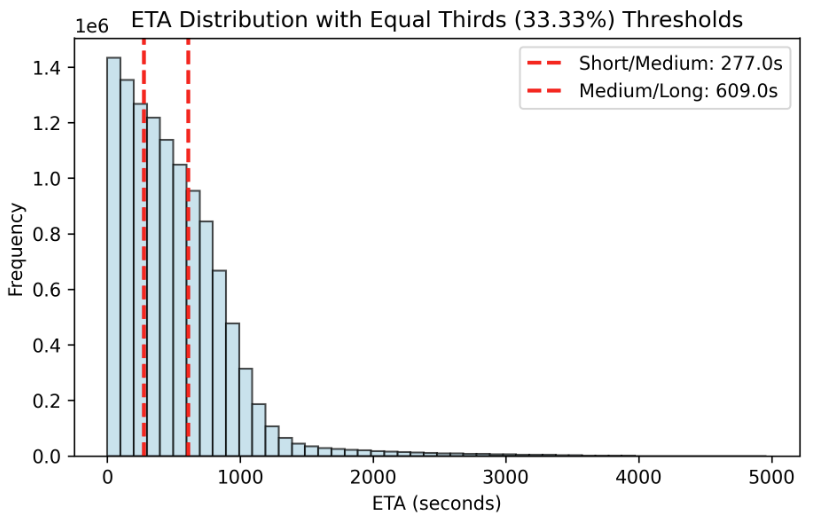
\includegraphics[width=0.95\linewidth]{figures/eta_dist.png}}{\fbox{\parbox{0.9\linewidth}{\centering ETA histogram placeholder}}}
    \caption{ETA distribution (seconds) with equal-thirds thresholds. Vertical dashed lines indicate short/medium ($\approx$277 s) and medium/long ($\approx$609 s) boundaries.}
    \label{fig:eta-dist}
\end{figure}

\begin{figure}[t]
    \centering
    \IfFileExists{figures/eta_box.png}{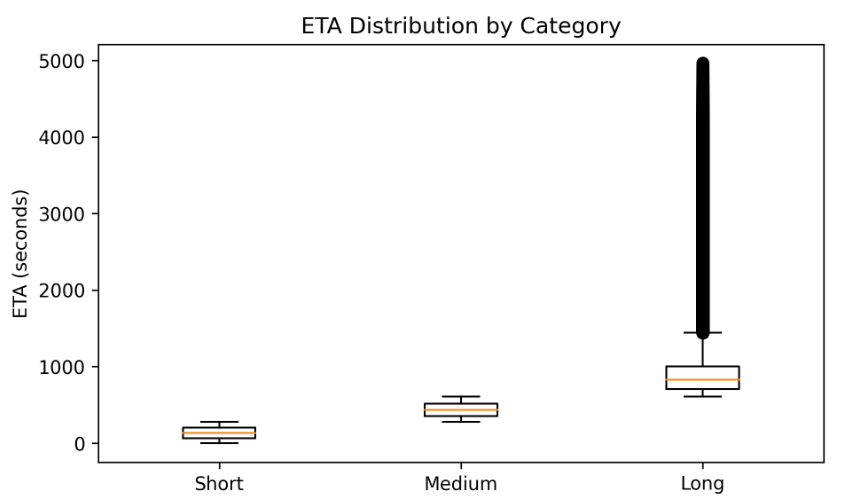
\includegraphics[width=0.95\linewidth]{figures/eta_box.png}}{\fbox{\parbox{0.9\linewidth}{\centering Boxplot placeholder}}}
    \caption{ETA distribution by route-length category (short/medium/long). Boxes summarize medians and IQRs; whiskers capture spread and outliers.}
    \label{fig:eta-box}
\end{figure}

\begin{figure}[t]
    \centering
    \IfFileExists{figures/eta_per_hour.png}{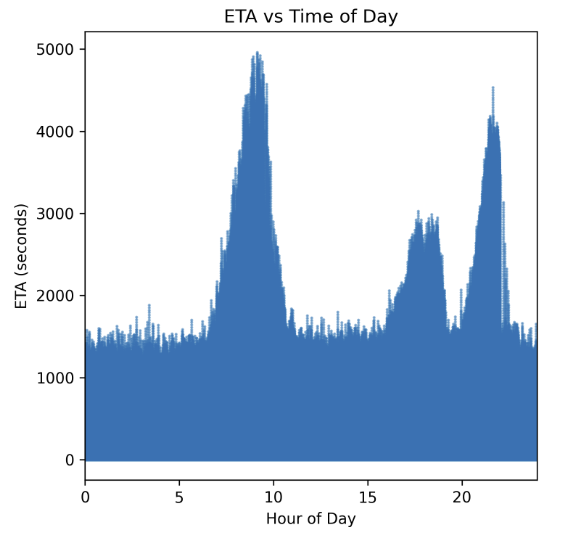
\includegraphics[width=0.95\linewidth]{figures/eta_per_hour.png}}{\fbox{\parbox{0.9\linewidth}{\centering Per-hour plot placeholder}}}
    \caption{ETA versus hour-of-day showing strong diurnal effects (morning and evening peaks), with occasional evening events/spikes.}
    \label{fig:eta-per-hour}
\end{figure}

\subsection{Experimental Setup}
Models are trained using AdamW with learning rate $10^{-3}$ and weight decay $10^{-2}$, batch size 2, for 200 epochs. The schedule uses a short linear warmup followed by cosine annealing ($T_{\text{max}}{=}200$). Targets are learned in a normalized space (default $y_{\text{log\_z}}$), while metrics are computed after consistent inversion to seconds. The router uses load-balancing (weight 0.05) and KL-to-uniform regularization (weight 0.002). Unless stated otherwise, reported numbers are the mean over seeds 42, 43, and 44; model selection uses the lowest validation MAE per seed.

\subsection{Baselines and Ablations}
We compare six code-defined variants (shared encoder and training protocol). Table~\ref{tab:ablation_variants} summarizes the variants and which components are enabled:
\begin{itemize}
    \item \texttt{base\_graph}: static road graph only; no dynamic edges; no temporal; no route features.
    \item \texttt{dynamic\_graph}: adds dynamic edges (junction$\to$vehicle, vehicle$\to$vehicle, vehicle$\to$junction); no temporal; no route features.
    \item \texttt{route\_aware\_graph}: adds route features/encoder and dynamic edges; no temporal.
    \item \texttt{temporal\_base}: temporal context from static-road edges only for the first $H{-}1$ snapshots; no route features; spatial encoder uses only static edges.
    \item \texttt{temporal\_dynamic}: temporal context from the first $H{-}1$ snapshots is aggregated over static-road edges; spatial encoder uses dynamic edges; no route features.
    \item \texttt{temporal\_route\_aware}: full model with dynamic edges, route features/encoder, and temporal context aggregated from static-road edges for the first $H{-}1$ snapshots.
\end{itemize}

\begin{table}[t]
    \centering
    \caption{Ablation variants and enabled components. Temporal uses a Transformer with static-road context for the first $H{-}1$ snapshots.}
    \label{tab:ablation_variants}
    \resizebox{\columnwidth}{!}{
    \begin{tabular}{@{}lccc@{}}
        \toprule
        \textbf{Variant} & \textbf{Dyn. Edges} & \textbf{Route Feat.} & \textbf{Temporal} \\
        \midrule
        base\_graph              & --- & --- & --- \\
        dynamic\_graph           & $\checkmark$ & --- & --- \\
        route\_aware\_graph      & $\checkmark$ & $\checkmark$ & --- \\
        temporal\_base           & --- & --- & $\checkmark$ \\
        temporal\_dynamic        & $\checkmark$ & --- & $\checkmark$ \\
        temporal\_route\_aware    & $\checkmark$ & $\checkmark$ & $\checkmark$ \\
        \bottomrule
    \end{tabular}}
\end{table}

\subsection{Evaluation Metrics}
We report Mean Absolute Error (MAE) and Root Mean Squared Error (RMSE) in seconds, and Mean Absolute Percentage Error (MAPE). We also provide stratified MAE by route-length and duration bins.


